\chapter{背景}
第2章ではグループ B で調査した新聞の背景について紹介する。新聞の現状における課題点やニュース砂漠、The New York Timesなどの実例を調査した。
\section{現状における問題点}
% 担当:中川翔真
% 背景や目的から現れた問題点を記述する。
グループBでは主に2つの課題が挙げられた。1つ目は、新聞の購読者数が年々減少していることである。特に若者の新聞離れが起きている。2つ目は、地方の新聞紙が無くなるニュース砂漠という現象が起きていることである。ニュース砂漠によって、地方の新聞が減少し、地元の情報を知る機会が減少する。これらの問題から、新聞記事には信頼性の高い情報が含まれているにもかかわらず購読者は減少し続けている。結果として、人々に十分な情報が届かなくなると考えられる。
\bunseki{中川翔真}

\section{実例に対する調査}
% 担当:伊藤太一、小山内魁人
% ニュース砂漠やThe New York Timesの実例に触れた経緯や結果などを記述する。
\subsection{購読者数の推移}
日本新聞協会によると、一般紙とスポーツ紙を合わせ、朝刊夕刊をセットとした発行部数は2000 年では53,708,831部であった[1]。しかし、2020 年では35,091,944 部と約20,000,000 部減少していることが分かった。また、2000 年時点では世帯数が47,419,905 世帯であったが、2020 年では57,380,526 世帯と約10,000,000 世帯増加している(図2.1)。これらの結果から、2000 年では1世帯あたりの部数は1.13 部であるのに対し、2020 年では0.61 部数と約54\%減少していることがわかる。よって、世帯数が年々増加しているにも関わらず、1 世帯当たりの部数が減少していることが問題と言えるだろう。\\
 総務省が公開している「主なメディアの利用時間と行為者率」[2]から、若者の新聞に対する関心がないと考えられる。総務省のデータをもとにグラフ化したものを下記に示す(図2.2、図2.3)。2015年のインターネットの利用時間では、平日において10代は112分、20代は146分である。これに対し2019年の場合では10代は167分であり、20代では177分となっている。年代ごとのインターネットの利用時間を比べると、10代では55分、20代では31分増加している。このことから、インターネットの利用時間は増加傾向にあることがわかる。また、2015年の新聞閲読時間は平日において、10代は0.2分、20代では2.1分であり、2019年の場合では10代は0.3分、20代では1.8分となっている。年代ごとの新聞閲読時間を比較すると、その差は1分程度となっており、ほぼ変化が無い。上記の調査結果から、インターネットの利用時間に比べ新聞閲読時間が圧倒的に短いことがわかる。よって、若者の関心は新聞ではなくインターネットにあると言える。
\newpage
\begin{figure}[htbp]
    \centering
    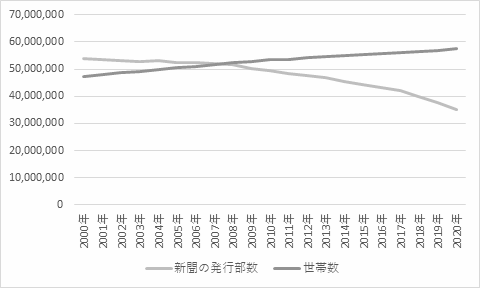
\includegraphics[keepaspectratio, scale=0.35]{images/newspaper1.png}
    \caption{新聞の発行部数と世帯数の推移}
    \label{fig:my_label}
\end{figure}

\begin{figure}[htbp]
    \begin{minipage}[b]{0.45\linewidth}
        \centering
        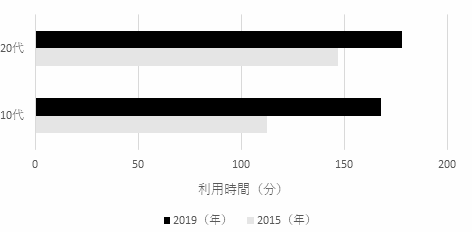
\includegraphics[keepaspectratio, scale=0.35]{images/newspaper2.png}
        \caption{インターネットの年代別利用時間}
    \end{minipage}
    \begin{minipage}[b]{0.45\linewidth}
        \centering
        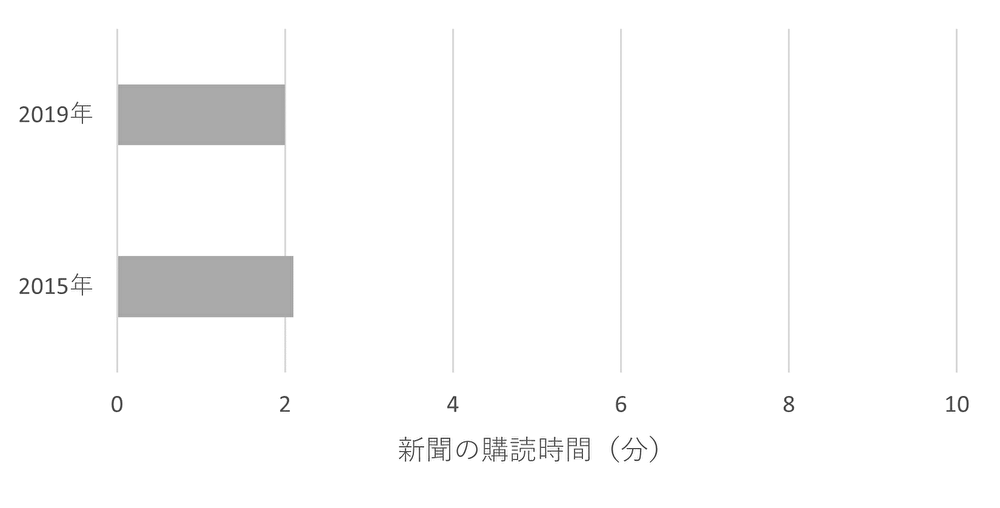
\includegraphics[keepaspectratio, scale=0.35]{images/newspaper3.png}
        \caption{新聞の年代別閲読時間 }
    \end{minipage}
\end{figure}
\bunseki{伊藤太一}

\subsection{ニュース砂漠}
ニュース砂漠とは地元に新聞社が0社、または1社であることを指す。実例として、アメリカのノースカロライナ大学の調査によると、アメリカの新聞社のうち 2004 年と比較し 2018 年では 1800 紙が廃刊に追い込まれている。また、ビューリサーチセンターによると2004年から2017年にかけて、新聞社に勤務する記者数が半減している[3]。北海道では、北海道新聞のほか、函館新聞や旭川新聞などの地方紙が存在する。その一方で 2021 年3月には地方夕刊紙である根室新聞が休刊に追い込まれた[4]。以上より、地方の人々が地元の情報を適切に得ることができなくなっている現状が発見された。
\bunseki{小山内魁人}

\subsection{The New York Times での実例}
The New York Timesでは、電子版のコンテンツとして、クロスワードパズルを導入している。その結果クロスワードパズルを含むコンテンツを目当てとした購読者数が2020年では110万人に達している[5]。
\bunseki{伊藤太一}